\documentclass[a4paper, 11pt]{article}

\usepackage{parskip}
\usepackage{hyperref}
\hypersetup{ colorlinks, citecolor=green, filecolor=black, linkcolor=blue, urlcolor=blue } 

\usepackage{colortbl}

\usepackage{amsfonts}

\usepackage[left=2cm, right=2cm, top=2cm]{geometry}
\usepackage{float}
\usepackage{afterpage}
\usepackage{multirow}

\usepackage{gensymb}
\usepackage{amsmath}
\usepackage{graphicx}
\usepackage{textcomp}
\usepackage{enumitem}

\newcommand{\points}[1]{(\textbf{#1 marks}) }
\newcommand{\vecthree}[3]{\begin{pmatrix} #1 \\ #2 \\ #3 \end{pmatrix}}
\newcommand{\vecfour}[4]{\begin{pmatrix} #1 \\ #2 \\ #3 \\ #4\end{pmatrix}}
\newcommand{\mat}[1]{\boldsymbol { \mathsf{#1}} }

\DeclareMathOperator*{\argmax}{arg\,max}
\DeclareMathOperator*{\argmin}{arg\,min}
\newcommand{\norm}[1]{\lVert#1\rVert}
\newcommand{\R}{\mathbb{R}}

\definecolor{mycolor}{rgb}{0,0.6,0.5}

\title{CS340/MATH321 -- Geometrical modelling and numerical analysis \\ Group project 2}
\vspace{-10em}
\date{Fall 2019}
\author{Huda Feroz Ahmed \and Aiman Khan \and Muhammad Shahrom Ali}

\begin{document}
\maketitle  
\setlength{\parskip}{10pt}
\setlength{\parindent}{0pt}
\DeclareGraphicsExtensions{.pdf,.png,.gif,.jpg}


\section*{Answers}
\begin{enumerate}
    
\item \textbf{(50 points)} The following question asks you to explore and implement the equation \[\vec p(s, t) = \sum N_i(s, t) \vec p_i\] in two- and three-dimensions

\begin{enumerate}[label=\alph*.]
    \item \textbf{(3 points)} Draw all the linear and quadratic B\'{e}zier basis functions over a unit interval and a unit square
    \item \textbf{(3 points)} Draw a linear, quadratic, cubic, quartic b-splines basis functions in 1D over a uniform knot vector
    \item \textbf{(3 points)} Draw quadratic, cubic, and quartic B\'{e}zier curves by arbitrary defining the appropriate control points
    \item \textbf{(6 points)} The curve generated using B\'{e}zier basis functions do not usually pass through the control points. Derive new quadratic and cubic polynomial basis functions $N_i(t)$ which when linearly combined with the control points $\vec p_i$ will generate a curve which passes through the control points. Draw them and comment on potential advantages and disadvantages of these basis functions. You can define the control points arbitrarily. 
    \item \textbf{(6 points)} Now imagine you have a cubic B\'{e}zier curves $\vec P(t)$ and $\vec Q(t)$, derive the conditions on the control points such that the curves $\vec P(t)$ join the curve $\vec Q(t)$ with $C^1$ and with $C^2$ continuity. What is the continuity of the cubic B\'{e}zier curve $\vec P(t)$ by itself.
    \item \textbf{(9 points)} For part e), draw a figure which demonstrates that the curve $\vec P(t)$ joins the curve $\vec Q(t)$ with $C^1$ continuity. Draw a similar figure(s) which demonstrates that the curves join with $C^2$ continuity. The figure must be generated by some algorithm/function.
    \item \textbf{(9 points)} Repeat parts c-d for a single patch with tensor product structure
    \item \textbf{(2 points)} Consider two arbitrary tensor product quadratic B\'{e}zier patches $\vec P(s,t)$ and $\vec Q(s,t)$, describe (qualitatively or mathematically) the conditions for $C^1$ continuity along the edge at which they meet?  
    \item \textbf{(9 points)} Define arbitrary control points for patches $\vec P(s,t)$ and $\vec Q(s,t)$ and generate a figure which demonstrates whether the patches connects with $C^1$ continuity. The figure must be generated by some algorithm/function.
\end{enumerate}

\item \textbf{(10 points)} This question asks you to generate a curve defined by the control points using the quadratic B\'{e}zier basis functions. You are given a circle.txt file. It has 16 vertices and 8 faces (line elements). Figure \ref{fig:lineMesh} shows this mesh. Describe succinctly what you have done

\begin{figure}
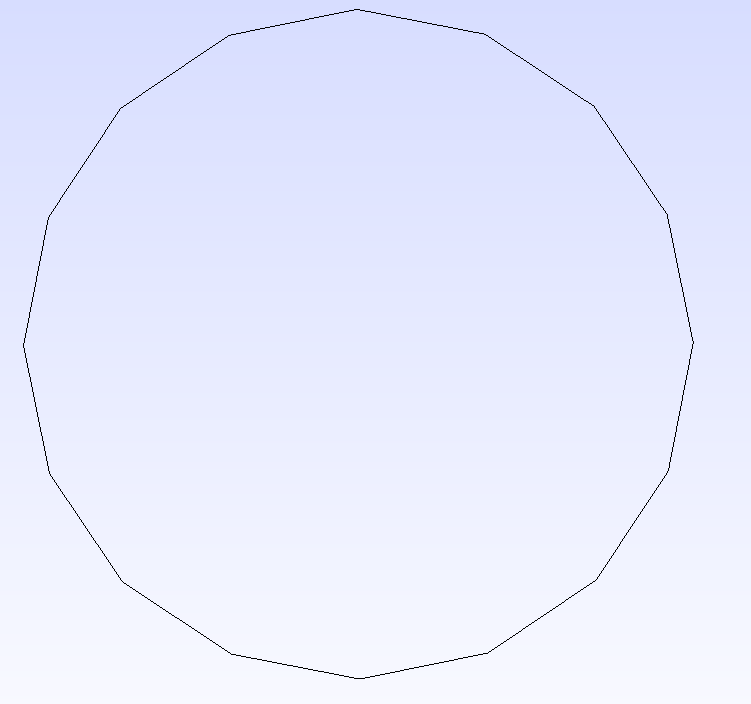
\includegraphics[scale=0.25]{resources/circleMesh.png} 
\centering
\caption{Line mesh of the circle}
\label{fig:lineMesh}
\end{figure}

Each face (element) of the mesh comprises of three vertices. For example circle.txt file shows that the second face comprises of vertices \{2, 3, 4\}. Using the parametrisation show in figure \ref{fig:lineElement}, generate the resulting geometry using the quadratic B\'{e}zier basis functions.
\begin{figure}
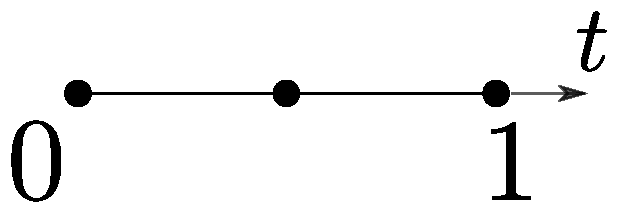
\includegraphics[scale=0.5]{resources/quadraticLineElement.pdf} 
\centering
\caption{Parametrisation of quadratic line element}
\label{fig:lineElement}
\end{figure}

\item \textbf{(20 points)} You are now asked to generalise your algorithm in question 2 from curves to surfaces. Given the mesh for the one-eighth of a sphere in sphere.txt. The screenshot of the mesh is shown in Figure \ref{fig:sphereFig}

\begin{figure}
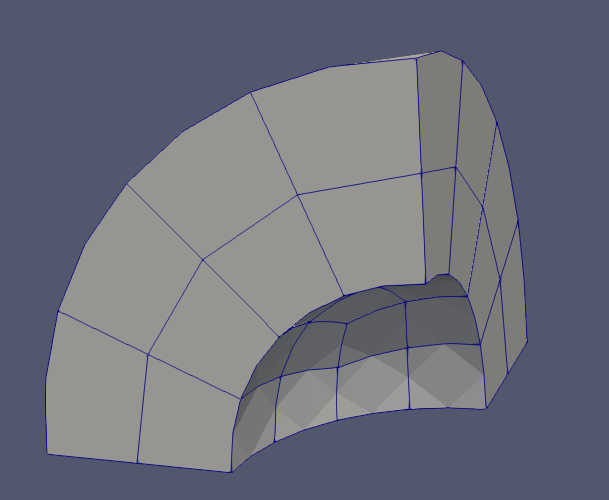
\includegraphics[scale=0.35]{resources/sphere.png} 
\centering
\caption{Mesh for the one-eighth of a sphere}
\label{fig:sphereFig}
\end{figure}

The 'sphere.txt' file has 224 vertices and 60 quadrilateral faces/elements. Each quadrilateral face/element comprises of 9 points. The quadrilateral in the sphere.txt numbers the vertices as shown in figure \ref{fig:sphereNodeNumber}. Generate the surface represented by the mesh  using the quadratic B\'{e}zier basis functions
\begin{figure}
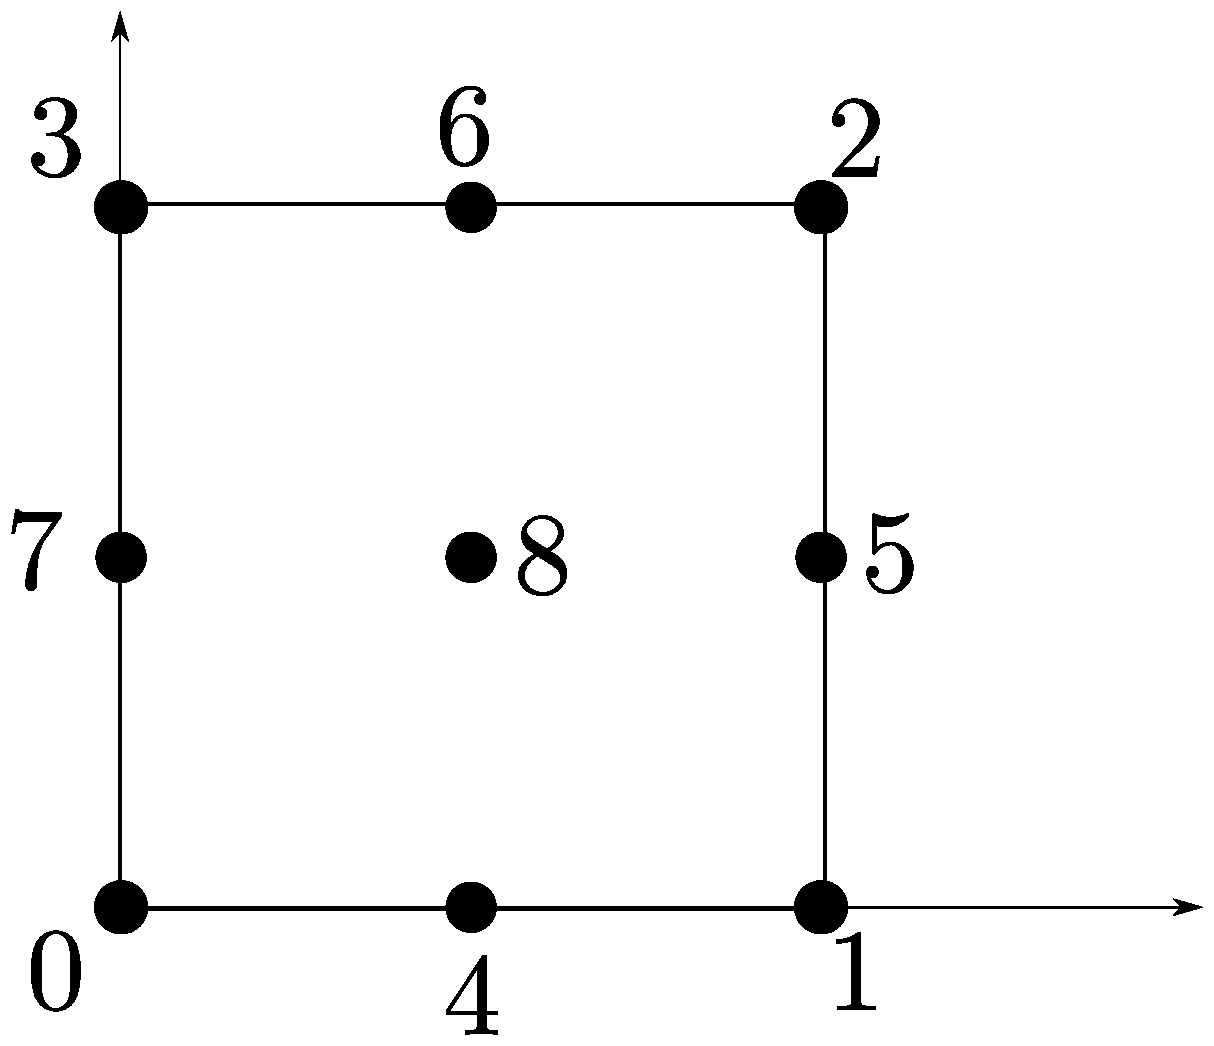
\includegraphics[scale=0.35]{resources/quadraticSquareElement.pdf} 
\centering
\caption{Mesh for the one-eighth of a sphere}
\label{fig:sphereNodeNumber} 
\end{figure}

\newpage

\section{Appendix A}
	
	\begin{verbatim}
	    Write Code here if you wanna.
	\end{verbatim}

\newpage

\begin{thebibliography}{9}
	\bibitem {testBIBI} Test Item. Remove this please 
		
	\begin{verbatim}
	    testing Capabilities. Remove this when adding the first Reference Item
	\end{verbatim}

\end{thebibliography}


\end{enumerate}
\end{document}
